\section{Datenlogger}

\begin{frame}
	\frametitle{Hardware}	
	\begin{columns}
		\begin{column}{0.6 \textwidth}
			\begin{itemize}
				\item VDIP1-Board von FTDI
				\item Daten auf USB-Stick speichern und lesen
				\item UART-Schnittstelle
			\end{itemize}
		\end{column}
		\begin{column}{0.4 \textwidth}
			\vspace{-2.8em}
			\begin{figure}[h]
				\centering
				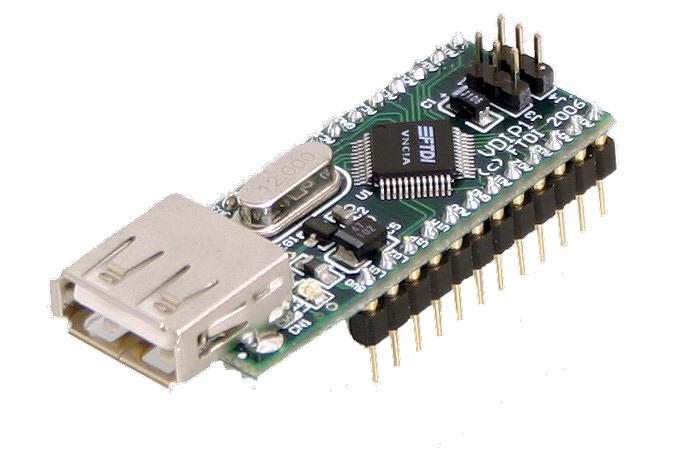
\includegraphics[width = 0.8 \textwidth]{../images/vdip1.jpg}
			\end{figure}
		\end{column}
	\end{columns}
\end{frame}

\begin{frame}
	\frametitle{Software}	
	\begin{itemize}
		\item Steuerung über einfache Befehle
		\item Initialisierung
		\item Ereignisse loggen
		\item Konfigurationsdaten lesen und speichern
		\item CSV-Format
	\end{itemize}
\end{frame}

\begin{frame}	
	\frametitle{Probleme}
	\begin{itemize}
		\item Log-Datei wird nicht geschlossen
		\item Absturz des Loggers
	\end{itemize}
	
\end{frame}